\section{Introduction}
\iLaTeX{} is a research prototype of a new kind of editor for \LaTeX{} documents.
It is built on top of \vsc, an open-source code editor.
\iLaTeX{} looks and works like other \LaTeX{} editors such as TeXstudio and Overleaf (\autoref{fig:ilatex-ui}), but it also offers a new kind of features we call \emph{interactive intermediate representations}---or IIR for short.

IIRs constitute an alternative way to visualise and manipulate certain parts of a \LaTeX{} document than the source code or the generated PDF.
Each IIR is bound to a piece of \emph{visualisable code}, \ie code that can be visualised through an IIR.

IIRs are an optional feature of \iLaTeX{}: since the source code of your documents remains accessible at all times, you can also use \iLaTeX{} like a standard \LaTeX{} editor and simply edit the code.
While \iLaTeX{} may not always be able to parse and understand the code you write, in which case IIRs will be disabled, it will never prevent you from compiling a \LaTeX{} document whose code is accepted by the \LaTeX{} compiler itself.

\begin{figure}[h]
    \centering
    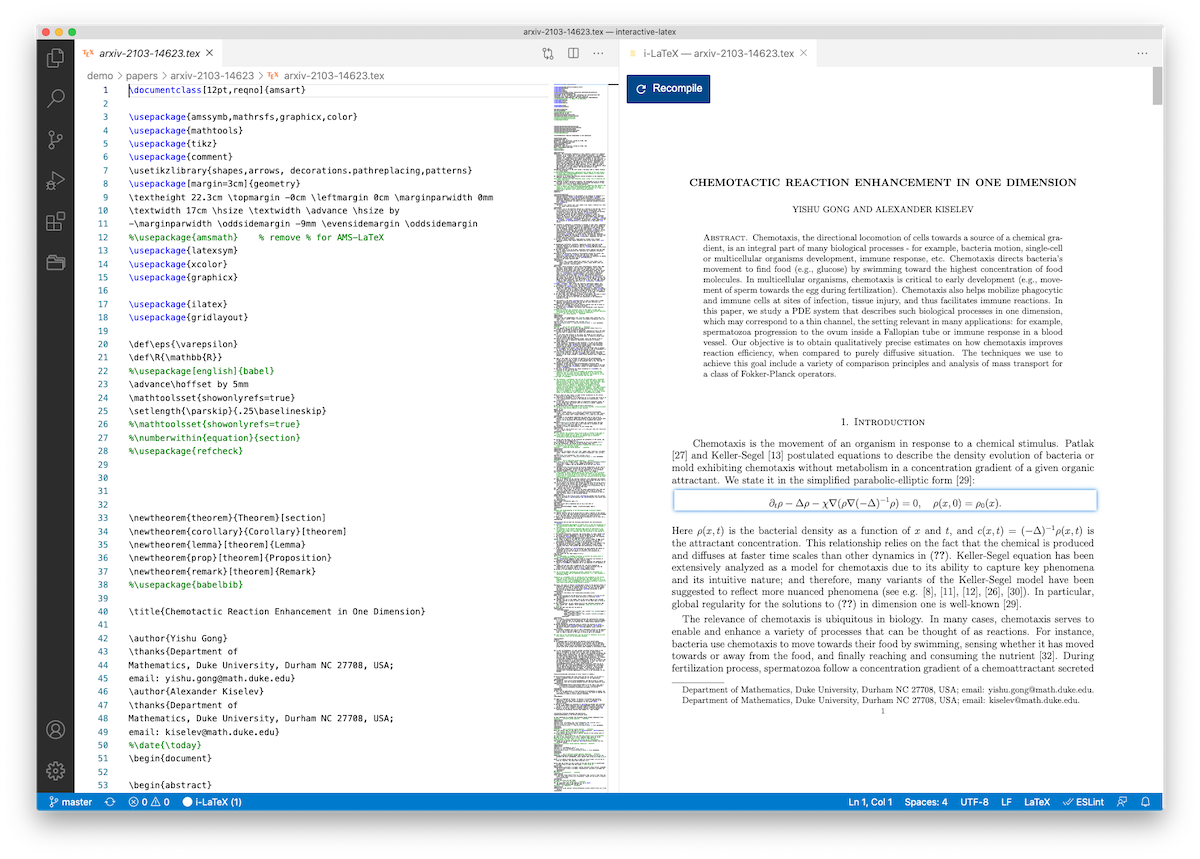
\includegraphics[width = \textwidth]{img/ilatex-editor-ui.png}
    \caption{A typical layout to edit a \LaTeX{} document opened with \iLaTeX{}: the code of the document is on the left, and the interactive PDF is on the right.}
    \label{fig:ilatex-ui}
\end{figure}